\chapter{Testing}\label{ch:tests}

Since we produce an executable, our output goes to \texttt{stdout}. This makes it somewhat roundabout to
try and use a particular language to test the outputs. Rather, we use \texttt{bash} to check if the produced
results are correct.

\section{Example Tests}
\subsection*{Fibonacci with cond}
\lstinputlisting[language=Lisp]{../test/class/fib-cond.rot}

\subsection*{Tail-call Fibonacci}
\lstinputlisting[language=Lisp]{../test/class/fib.rot}

\subsection*{Normal Factorial}
\lstinputlisting[language=Lisp]{../test/class/fact.rot}

\subsection*{Tail-call Factorial}
\lstinputlisting[language=Lisp]{../test/class/fact-tc.rot}

\subsection*{Find}
\lstinputlisting[language=Lisp]{../test/class/find.rot}

\subsection*{List}
\lstinputlisting[language=Lisp]{../test/class/list.rot}

\subsection*{Map}
\lstinputlisting[language=Lisp]{../test/class/map.rot}

\subsection*{Sort}
\lstinputlisting[language=Lisp]{../test/class/sort.rot}

\subsection*{Standard Library Test}
\lstinputlisting[language=Lisp]{../test/class/std-test.rot}
\clearpage

\subsection*{Mutually Recursive Lambdas}
\lstinputlisting[language=Lisp]{../test/lambdas/mrec.rot}

\subsection*{String Length}
\lstinputlisting[language=Lisp]{../test/strings/string-length.rot}

\subsection*{String Ref}
\lstinputlisting[language=Lisp]{../test/strings/string-ref.rot}

\subsection*{Multiple relational ops with begin}
\lstinputlisting[language=Lisp]{../test/prims/relop.rot}
\clearpage

\section{Example Test Outputs}
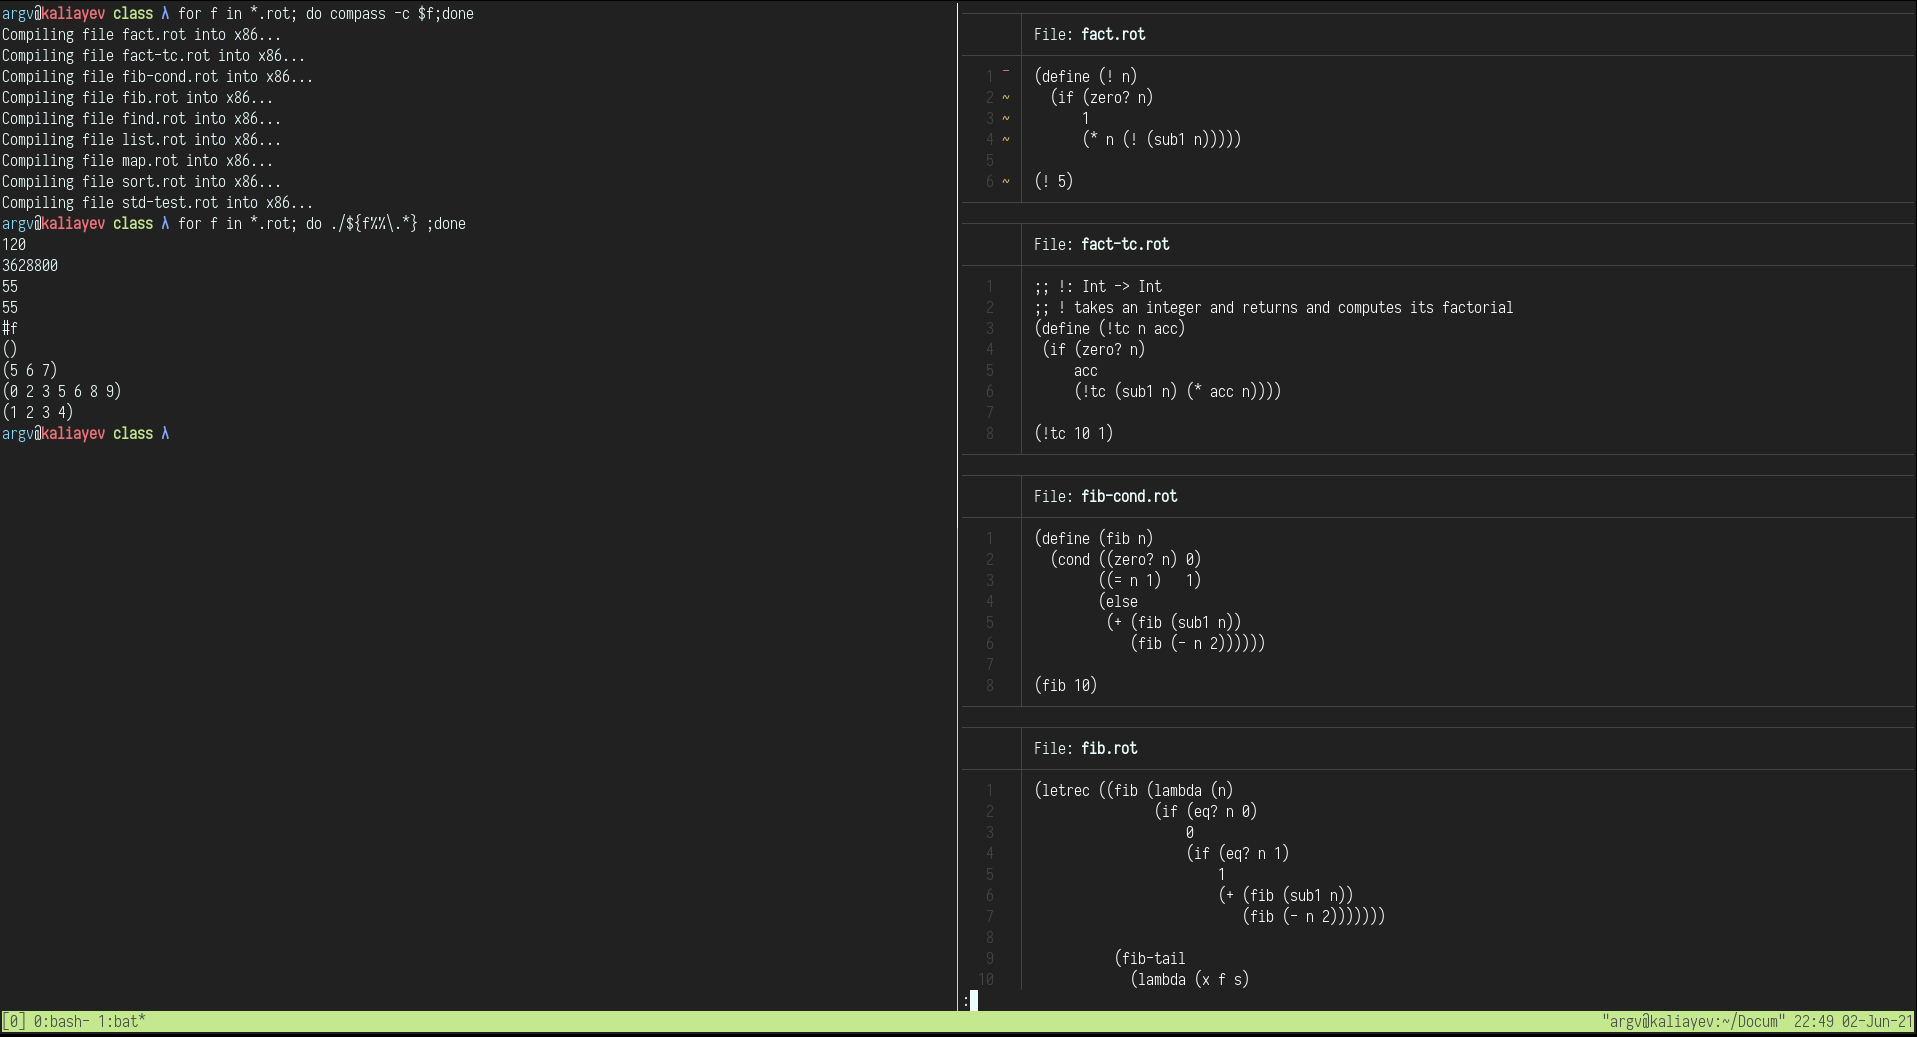
\includegraphics[width=0.8\paperwidth]{figures/ch4/test-run-1}
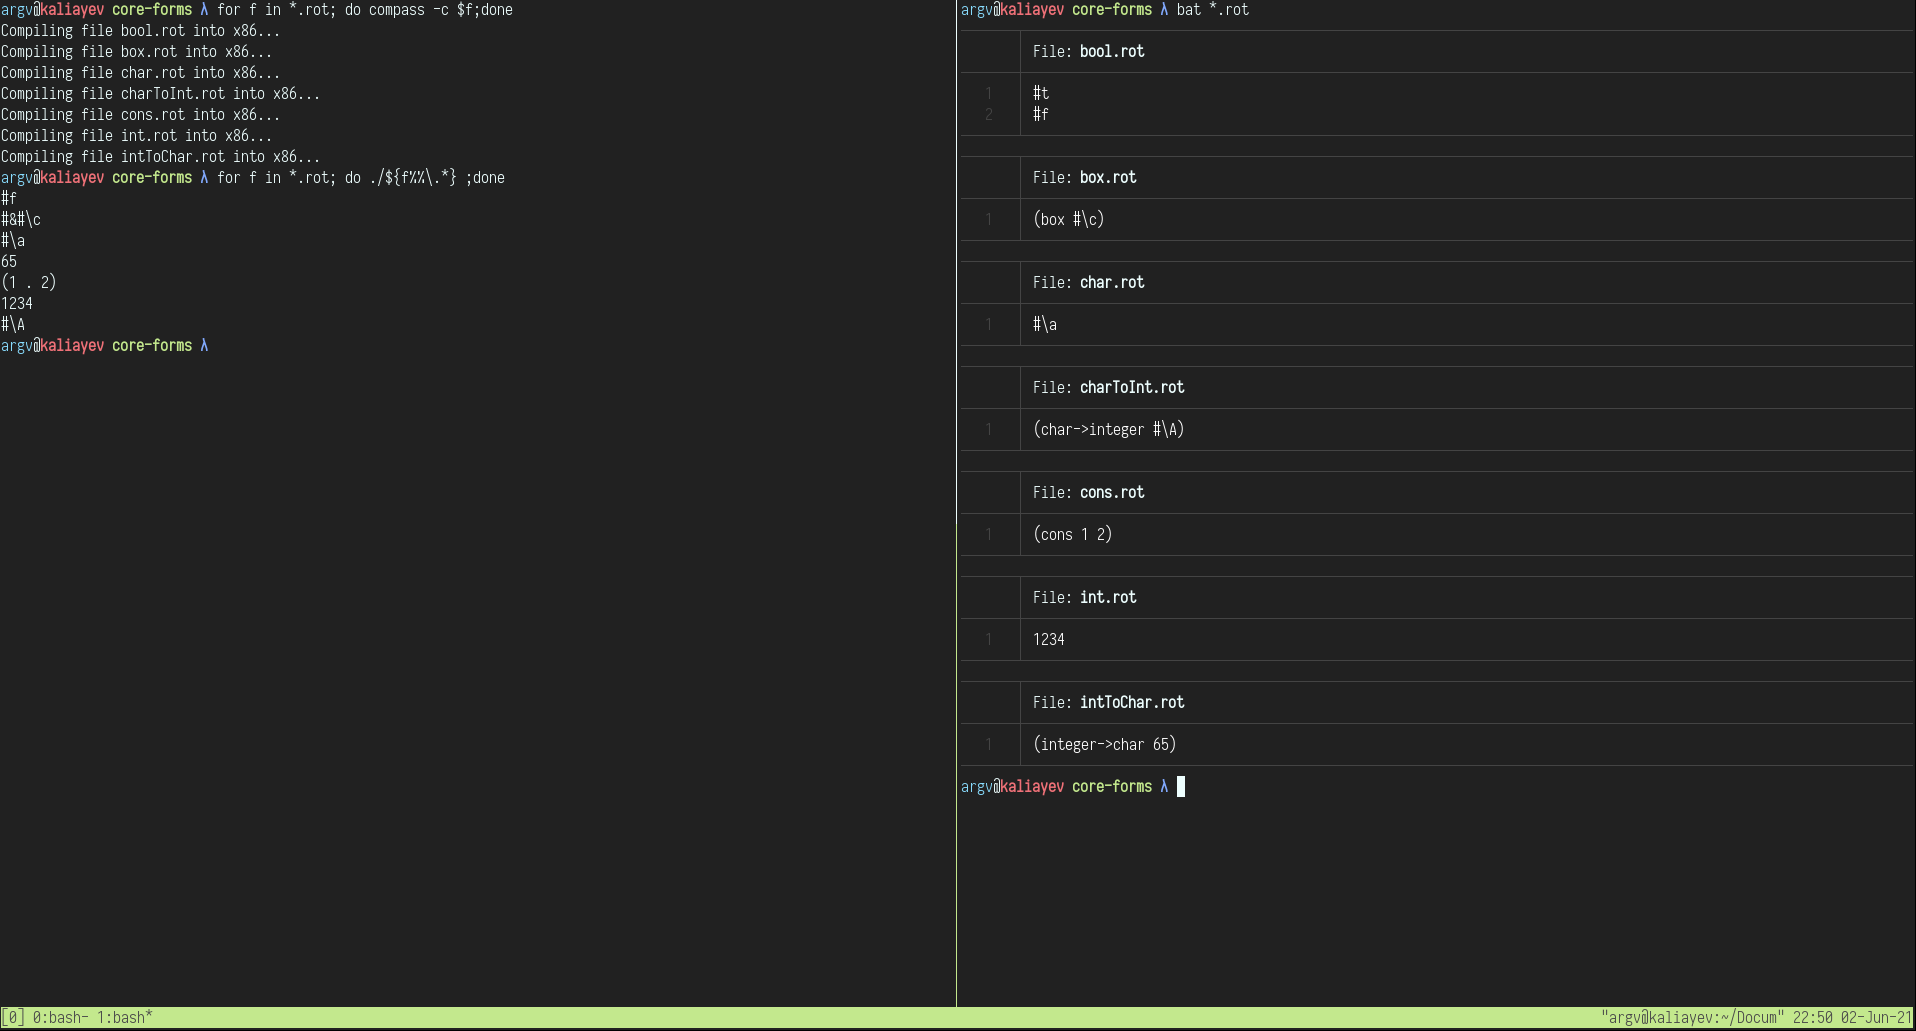
\includegraphics[width=0.8\paperwidth]{figures/ch4/test-run-2}
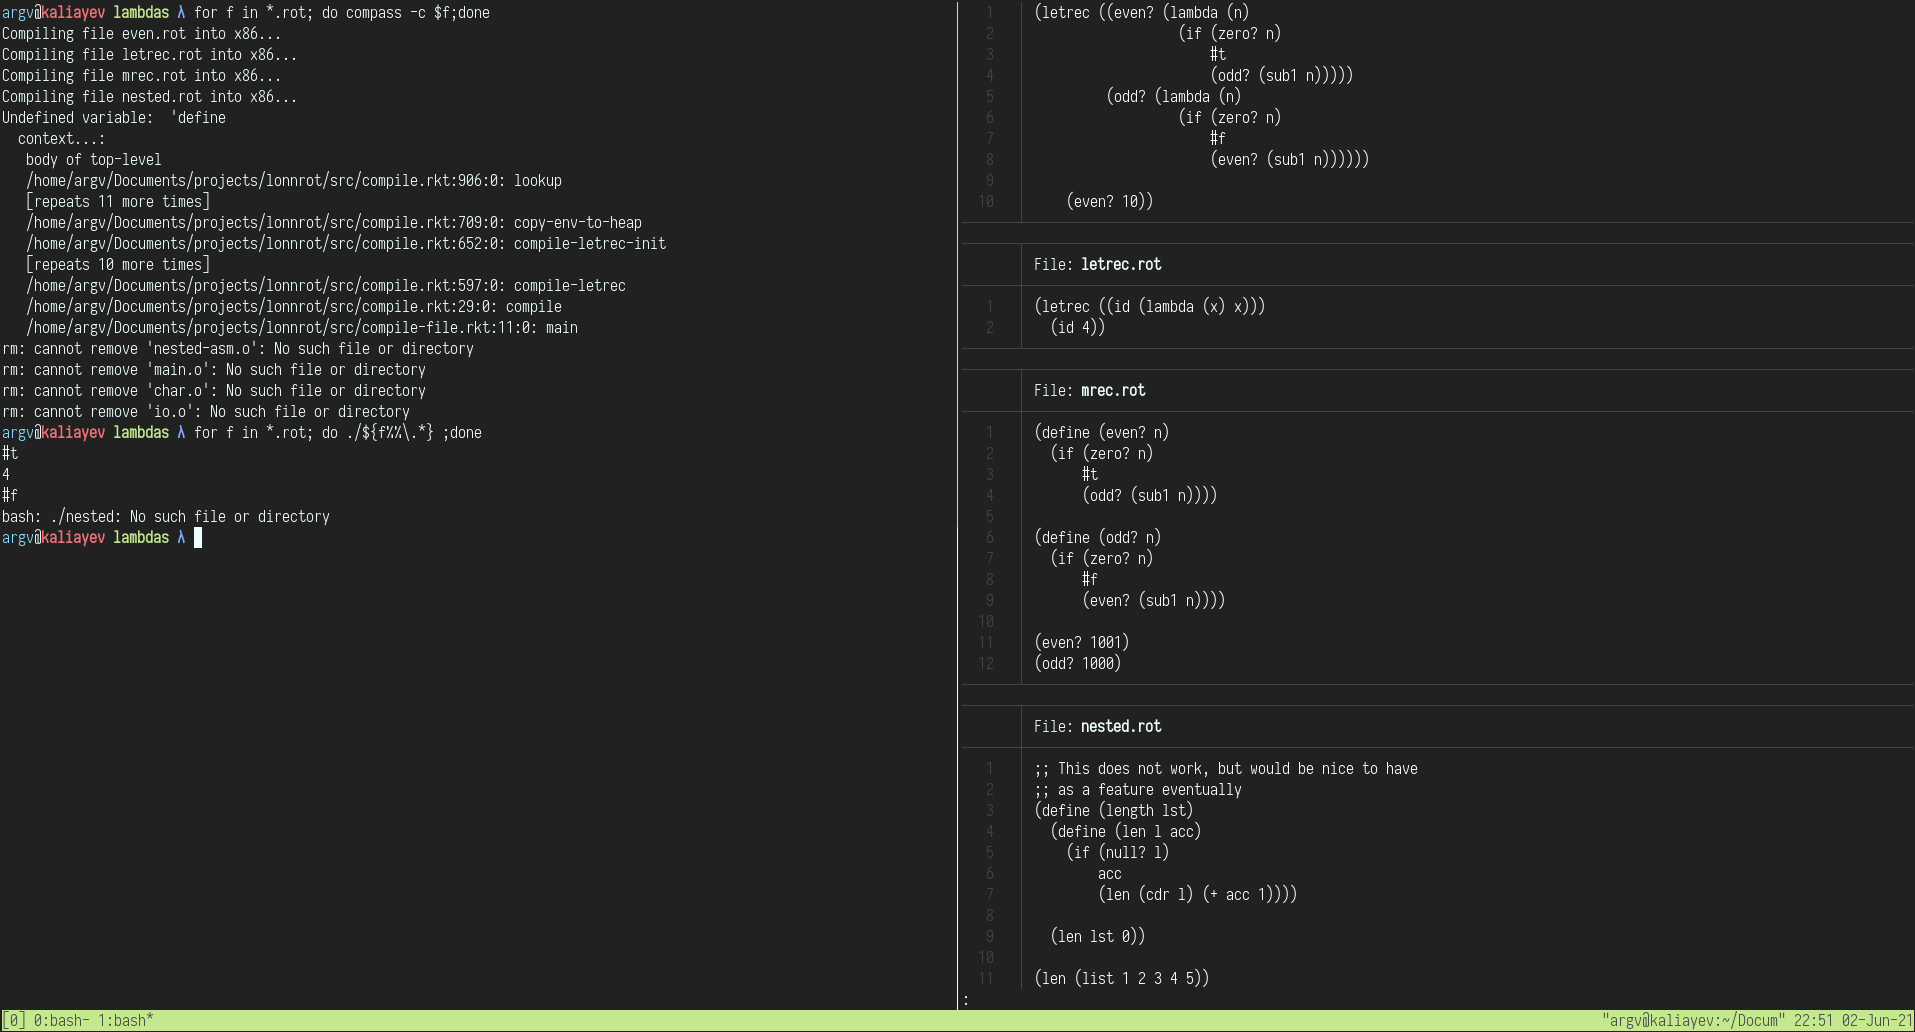
\includegraphics[width=0.8\paperwidth]{figures/ch4/test-run-3}
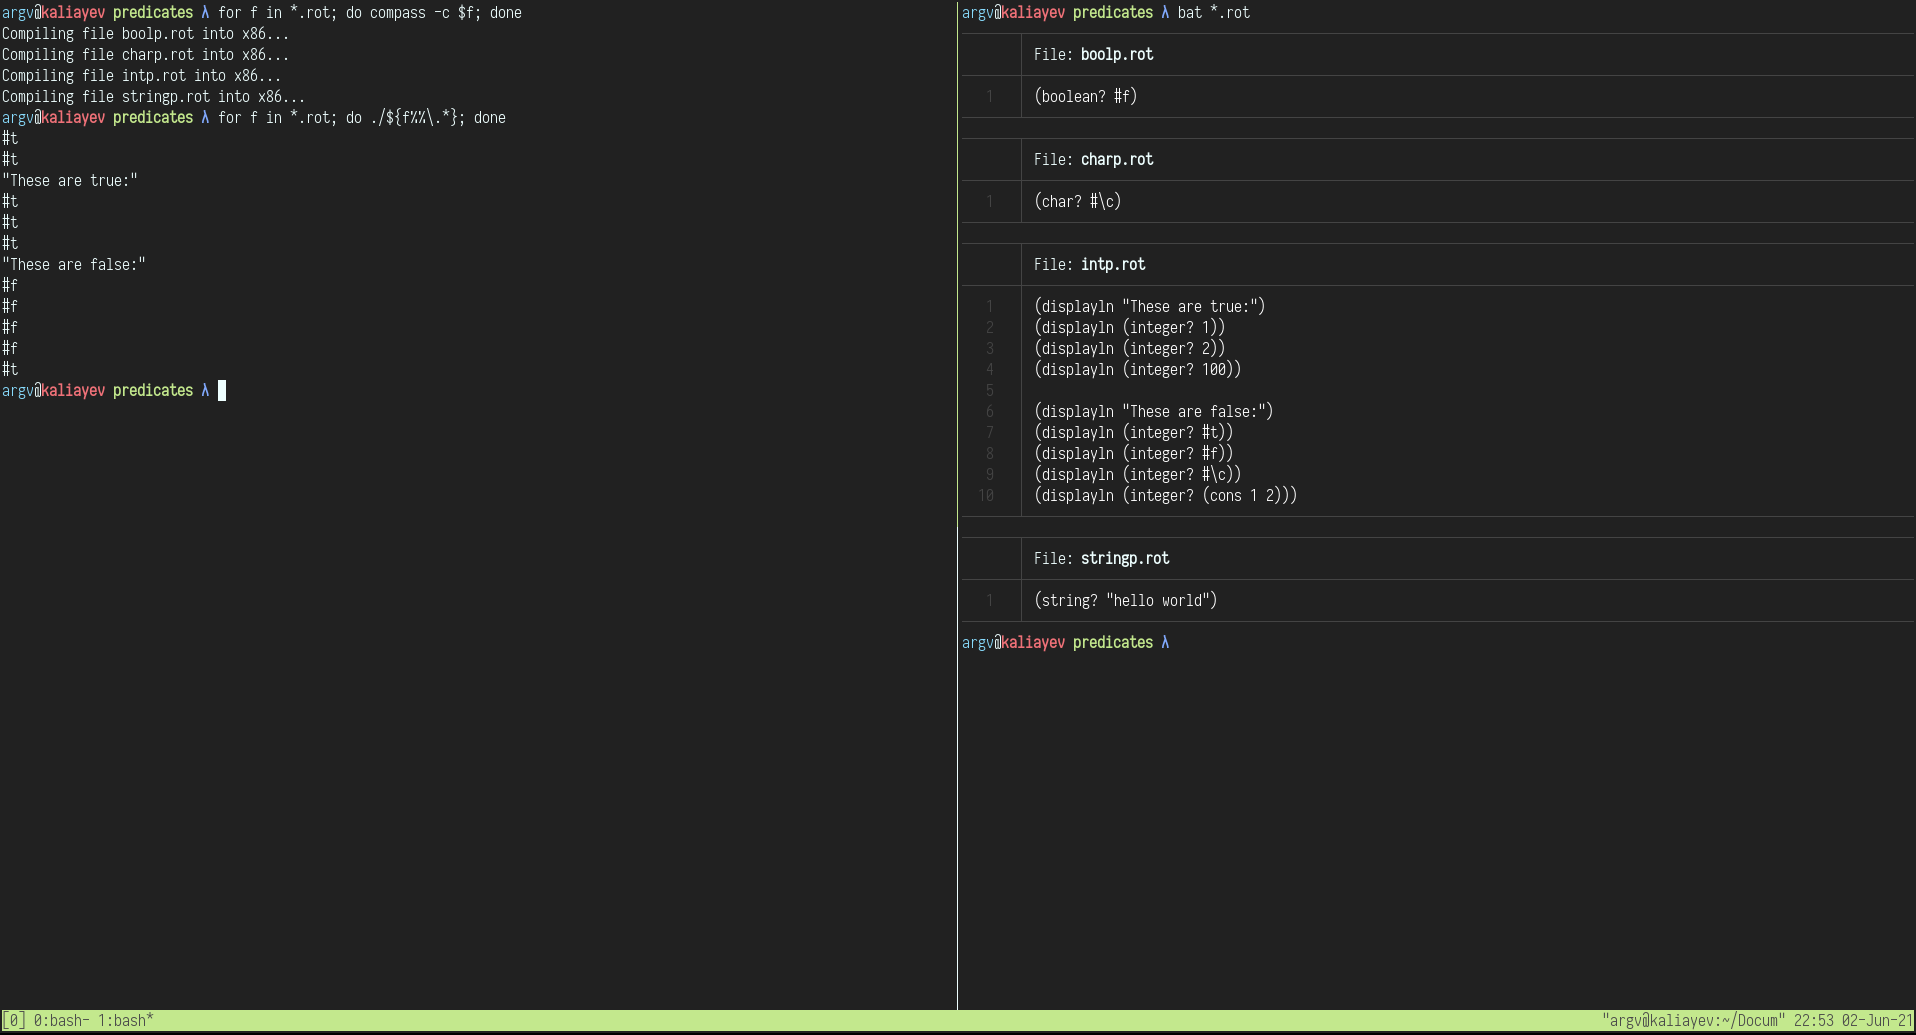
\includegraphics[width=0.8\paperwidth]{figures/ch4/test-run-4}
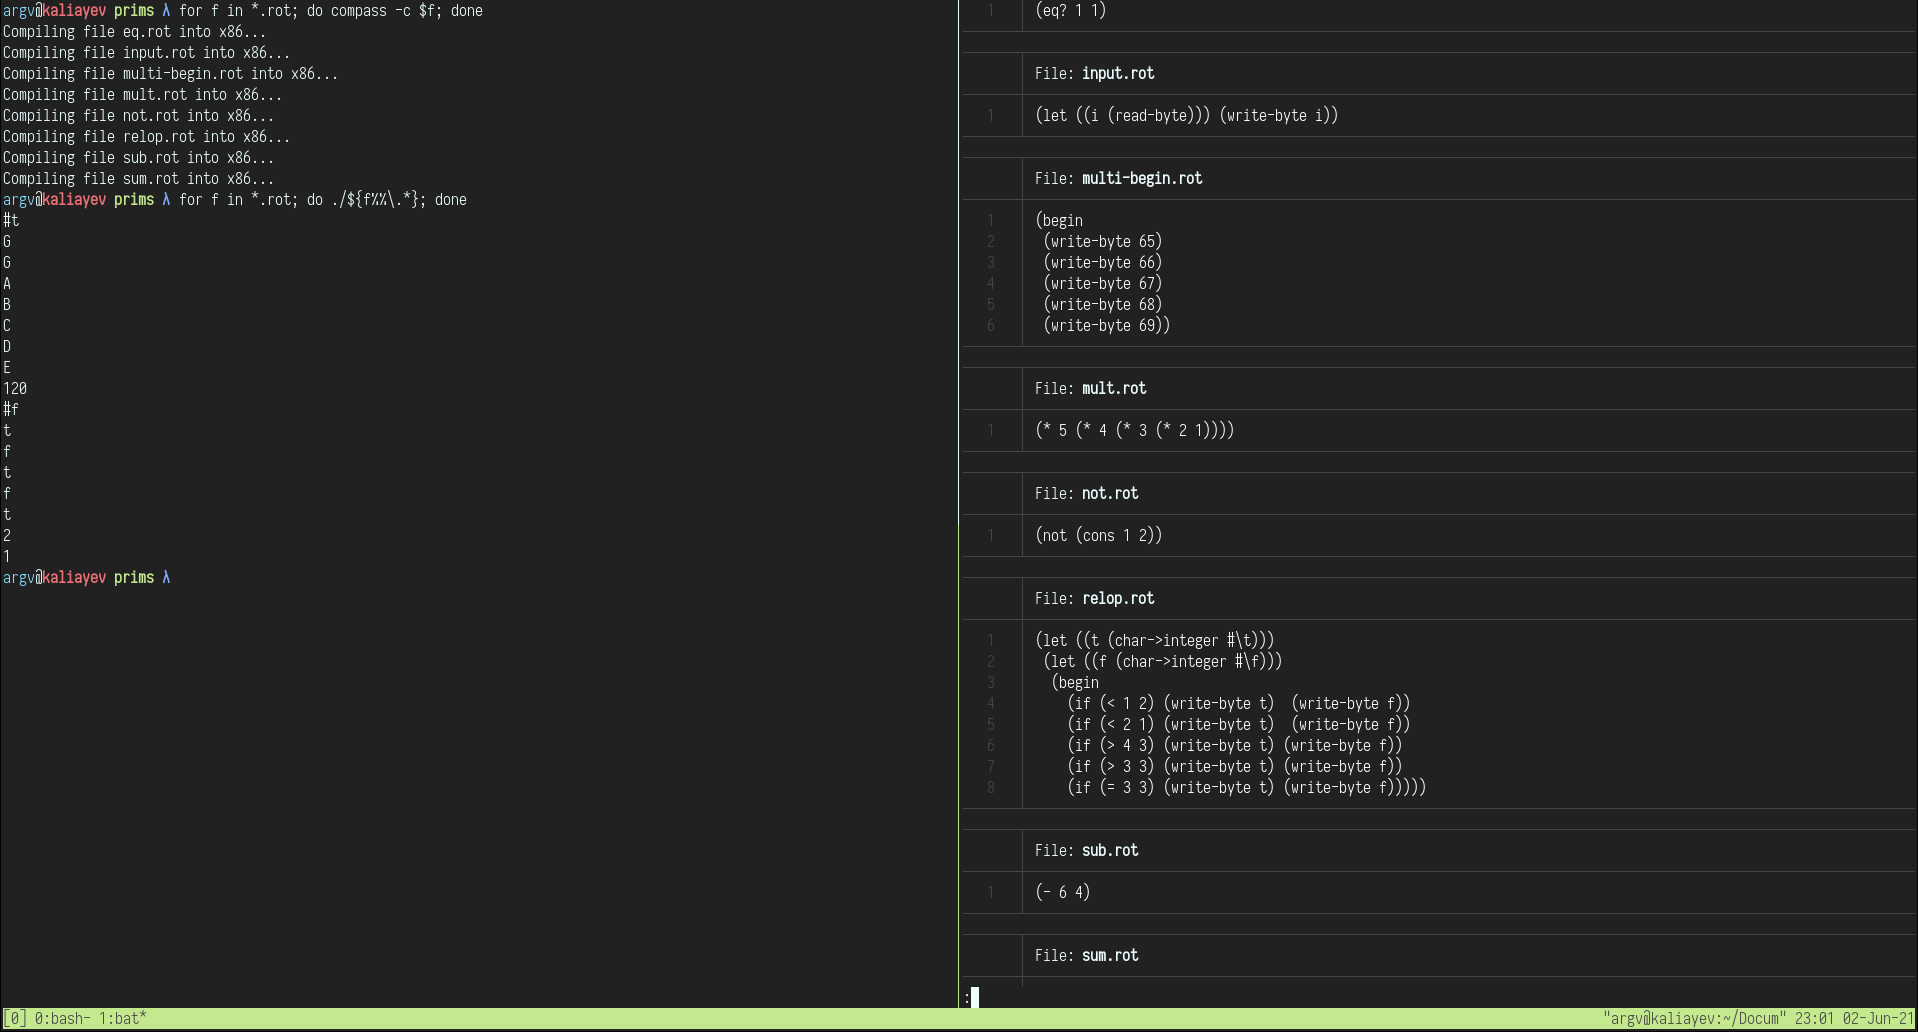
\includegraphics[width=0.8\paperwidth]{figures/ch4/test-run-5}
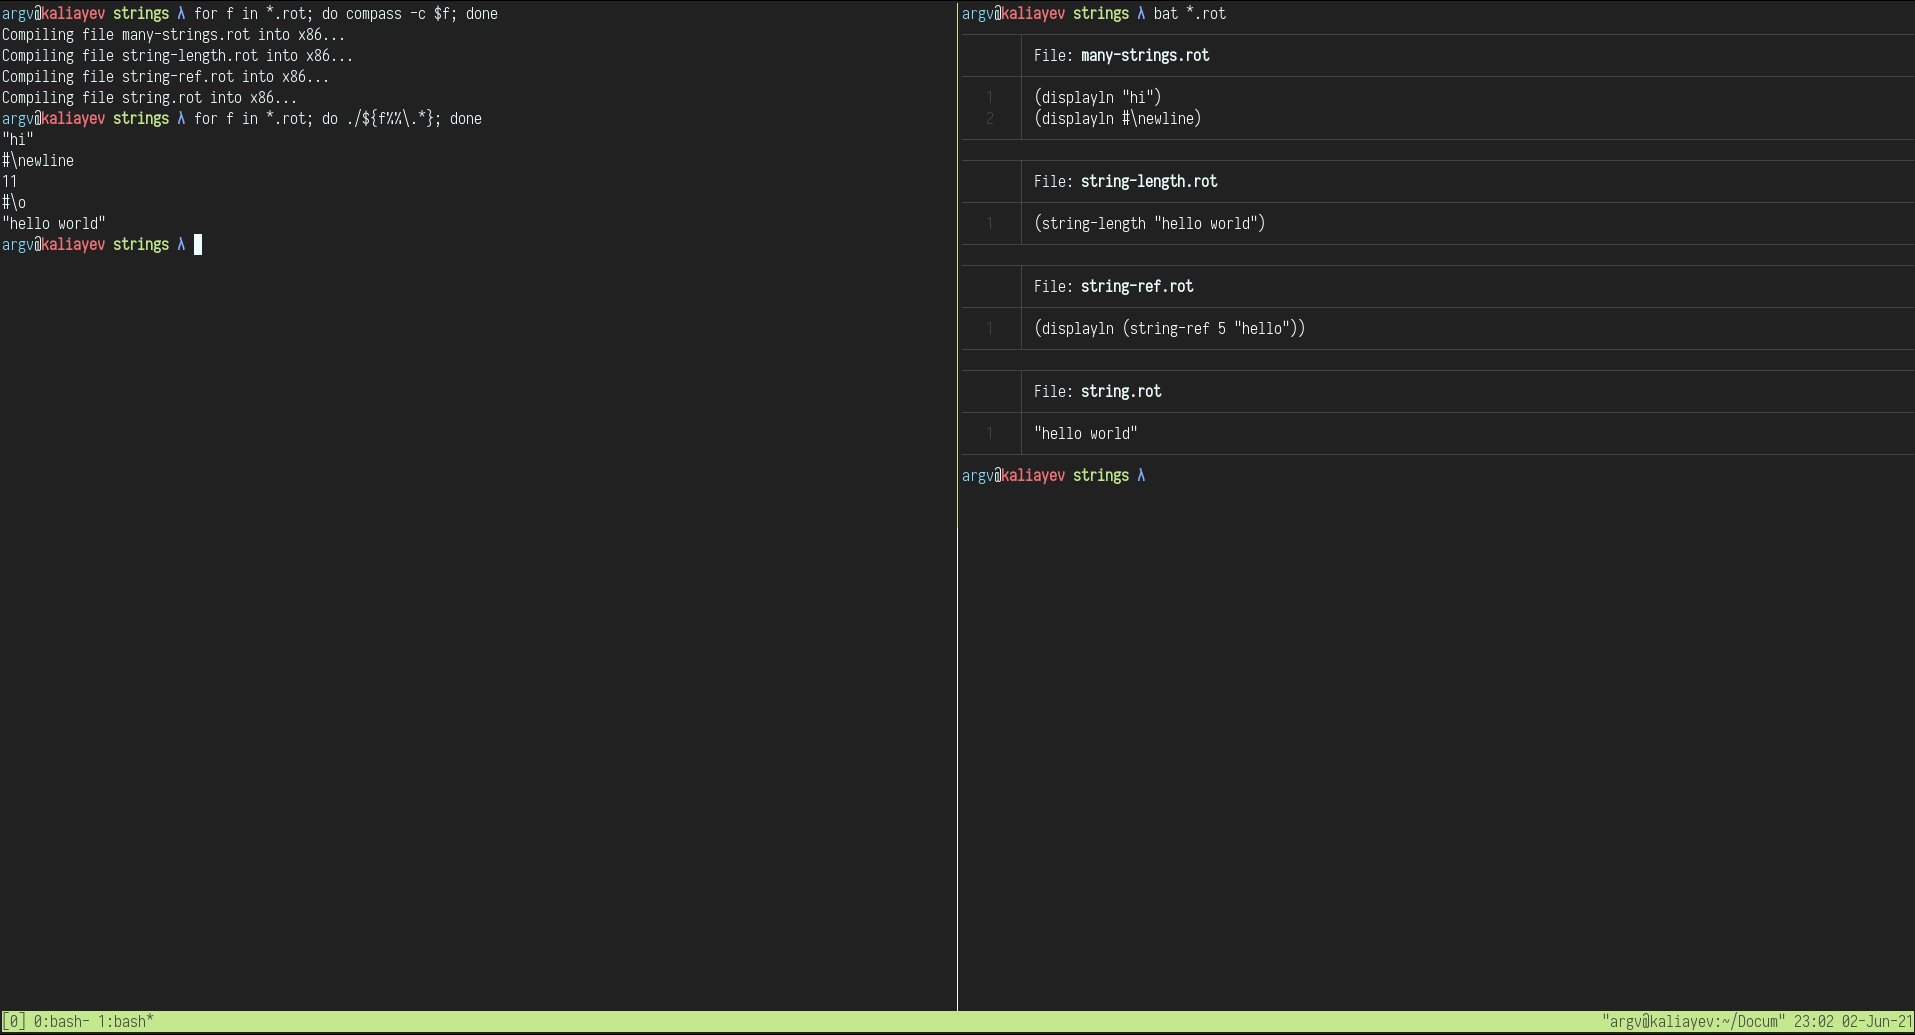
\includegraphics[width=0.8\paperwidth]{figures/ch4/test-run-6}
